\documentclass[11pt,a4paper]{article}
\usepackage[utf8]{inputenc}
\usepackage[T1]{fontenc}
\usepackage{lmodern}
\usepackage[margin=2.6cm]{geometry}
\usepackage{amsmath,amssymb,booktabs,graphicx,caption,setspace}
\usepackage[round,authoryear]{natbib}
\usepackage[hidelinks]{hyperref}
\graphicspath{{../figures/}}
\captionsetup{font=small,labelfont=bf}
\setstretch{1.12}
% generated by scripts/06_paper_assets.py -- do not edit
\newcommand{\regUnwFast}{0.55}
\newcommand{\pRegUnwFast}{0.010}
\newcommand{\regRbFast}{0.56}
\newcommand{\pRegRbFast}{0.009}
\newcommand{\regHbFast}{0.24}
\newcommand{\pRegHbFast}{0.040}
\newcommand{\hbEventNeg}{15.8}
\newcommand{\hbPlaceboNeg}{13.4}
\newcommand{\kurtPrec}{11}
\newcommand{\kurtHuber}{38}
\newcommand{\kurtPlain}{22}
\newcommand{\nSigDistrict}{1}
\newcommand{\slopeDistrictMainSlow}{\ensuremath{-}0.19}
\newcommand{\pSlopeDistrictMainSlow}{0.292}
\newcommand{\negSlopeDistrictMainSlow}{4}
\newcommand{\pSlopeDistrictMainSlowHolm}{1.000}
\newcommand{\slopeDistrictMainFast}{\ensuremath{-}0.27}
\newcommand{\pSlopeDistrictMainFast}{0.370}
\newcommand{\negSlopeDistrictMainFast}{3}
\newcommand{\pSlopeDistrictMainFastHolm}{1.000}
\newcommand{\slopeDistrictMainMid}{\ensuremath{-}0.01}
\newcommand{\pSlopeDistrictMainMid}{0.956}
\newcommand{\negSlopeDistrictMainMid}{2}
\newcommand{\pSlopeDistrictMainMidHolm}{1.000}
\newcommand{\slopeDistrictMainAll}{\ensuremath{-}0.03}
\newcommand{\pSlopeDistrictMainAll}{0.791}
\newcommand{\negSlopeDistrictMainAll}{2}
\newcommand{\pSlopeDistrictMainAllHolm}{1.000}
\newcommand{\slopeDistrictFarSlow}{\ensuremath{-}0.52}
\newcommand{\pSlopeDistrictFarSlow}{0.011}
\newcommand{\negSlopeDistrictFarSlow}{5}
\newcommand{\pSlopeDistrictFarSlowHolm}{0.112}
\newcommand{\slopeDistrictFarFast}{\ensuremath{-}0.23}
\newcommand{\pSlopeDistrictFarFast}{0.482}
\newcommand{\negSlopeDistrictFarFast}{3}
\newcommand{\pSlopeDistrictFarFastHolm}{1.000}
\newcommand{\slopeDistrictFarMid}{\ensuremath{-}0.22}
\newcommand{\pSlopeDistrictFarMid}{0.481}
\newcommand{\negSlopeDistrictFarMid}{4}
\newcommand{\pSlopeDistrictFarMidHolm}{1.000}
\newcommand{\slopeDistrictFarAll}{\ensuremath{-}0.30}
\newcommand{\pSlopeDistrictFarAll}{0.093}
\newcommand{\negSlopeDistrictFarAll}{4}
\newcommand{\pSlopeDistrictFarAllHolm}{0.932}
\newcommand{\nSigGeneral}{3}
\newcommand{\slopeGeneralMainSlow}{\ensuremath{-}0.60}
\newcommand{\pSlopeGeneralMainSlow}{0.009}
\newcommand{\negSlopeGeneralMainSlow}{4}
\newcommand{\pSlopeGeneralMainSlowHolm}{0.087}
\newcommand{\slopeGeneralMainFast}{\ensuremath{-}0.53}
\newcommand{\pSlopeGeneralMainFast}{0.227}
\newcommand{\negSlopeGeneralMainFast}{4}
\newcommand{\pSlopeGeneralMainFastHolm}{1.000}
\newcommand{\slopeGeneralMainMid}{\ensuremath{-}0.01}
\newcommand{\pSlopeGeneralMainMid}{0.980}
\newcommand{\negSlopeGeneralMainMid}{2}
\newcommand{\pSlopeGeneralMainMidHolm}{1.000}
\newcommand{\slopeGeneralMainAll}{\ensuremath{-}0.05}
\newcommand{\pSlopeGeneralMainAll}{0.747}
\newcommand{\negSlopeGeneralMainAll}{3}
\newcommand{\pSlopeGeneralMainAllHolm}{1.000}
\newcommand{\slopeGeneralFarSlow}{\ensuremath{-}1.08}
\newcommand{\pSlopeGeneralFarSlow}{0.0007}
\newcommand{\negSlopeGeneralFarSlow}{5}
\newcommand{\pSlopeGeneralFarSlowHolm}{0.007}
\newcommand{\slopeGeneralFarFast}{\ensuremath{-}0.70}
\newcommand{\pSlopeGeneralFarFast}{0.106}
\newcommand{\negSlopeGeneralFarFast}{5}
\newcommand{\pSlopeGeneralFarFastHolm}{1.000}
\newcommand{\slopeGeneralFarMid}{\ensuremath{-}0.12}
\newcommand{\pSlopeGeneralFarMid}{0.723}
\newcommand{\negSlopeGeneralFarMid}{4}
\newcommand{\pSlopeGeneralFarMidHolm}{1.000}
\newcommand{\slopeGeneralFarAll}{\ensuremath{-}0.37}
\newcommand{\pSlopeGeneralFarAll}{0.032}
\newcommand{\negSlopeGeneralFarAll}{5}
\newcommand{\pSlopeGeneralFarAllHolm}{0.318}
\newcommand{\nSigNeighbourhood}{2}
\newcommand{\slopeNeighbourhoodMainSlow}{\ensuremath{-}0.72}
\newcommand{\pSlopeNeighbourhoodMainSlow}{0.001}
\newcommand{\negSlopeNeighbourhoodMainSlow}{5}
\newcommand{\pSlopeNeighbourhoodMainSlowHolm}{0.014}
\newcommand{\slopeNeighbourhoodMainFast}{\ensuremath{-}0.66}
\newcommand{\pSlopeNeighbourhoodMainFast}{0.169}
\newcommand{\negSlopeNeighbourhoodMainFast}{4}
\newcommand{\pSlopeNeighbourhoodMainFastHolm}{1.000}
\newcommand{\slopeNeighbourhoodMainMid}{\ensuremath{-}0.04}
\newcommand{\pSlopeNeighbourhoodMainMid}{0.895}
\newcommand{\negSlopeNeighbourhoodMainMid}{2}
\newcommand{\pSlopeNeighbourhoodMainMidHolm}{1.000}
\newcommand{\slopeNeighbourhoodMainAll}{\ensuremath{-}0.04}
\newcommand{\pSlopeNeighbourhoodMainAll}{0.809}
\newcommand{\negSlopeNeighbourhoodMainAll}{3}
\newcommand{\pSlopeNeighbourhoodMainAllHolm}{1.000}
\newcommand{\slopeNeighbourhoodFarSlow}{\ensuremath{-}1.19}
\newcommand{\pSlopeNeighbourhoodFarSlow}{0.0004}
\newcommand{\negSlopeNeighbourhoodFarSlow}{5}
\newcommand{\pSlopeNeighbourhoodFarSlowHolm}{0.004}
\newcommand{\slopeNeighbourhoodFarFast}{\ensuremath{-}0.69}
\newcommand{\pSlopeNeighbourhoodFarFast}{0.144}
\newcommand{\negSlopeNeighbourhoodFarFast}{4}
\newcommand{\pSlopeNeighbourhoodFarFastHolm}{1.000}
\newcommand{\slopeNeighbourhoodFarMid}{\ensuremath{-}0.21}
\newcommand{\pSlopeNeighbourhoodFarMid}{0.540}
\newcommand{\negSlopeNeighbourhoodFarMid}{4}
\newcommand{\pSlopeNeighbourhoodFarMidHolm}{1.000}
\newcommand{\slopeNeighbourhoodFarAll}{\ensuremath{-}0.31}
\newcommand{\pSlopeNeighbourhoodFarAll}{0.085}
\newcommand{\negSlopeNeighbourhoodFarAll}{4}
\newcommand{\pSlopeNeighbourhoodFarAllHolm}{0.854}
\newcommand{\nSlopeTests}{10}
\newcommand{\pSideRegMin}{0.418}
\newcommand{\nCellsGeneral}{3\,030}
\newcommand{\sdChpGeneral}{12.1}
\newcommand{\nCellsMahalle}{3\,029}
\newcommand{\sdChpMahalle}{13.6}
\newcommand{\medMatched}{100}
\newcommand{\regMainAll}{0.05}
\newcommand{\pRegMainAll}{0.376}
\newcommand{\regMainFast}{0.57}
\newcommand{\pRegMainFast}{0.002}
\newcommand{\regMainSlow}{\ensuremath{-}0.04}
\newcommand{\pRegMainSlow}{0.561}
\newcommand{\regMainMid}{0.24}
\newcommand{\pRegMainMid}{0.115}
\newcommand{\regFarAll}{\ensuremath{-}0.03}
\newcommand{\pRegFarAll}{0.553}
\newcommand{\regFarFast}{0.41}
\newcommand{\pRegFarFast}{0.062}
\newcommand{\regFarSlow}{0.29}
\newcommand{\pRegFarSlow}{0.215}
\newcommand{\regFarMid}{0.24}
\newcommand{\pRegFarMid}{0.243}
\newcommand{\regPreAll}{\ensuremath{-}0.17}
\newcommand{\pRegPreAll}{0.792}
\newcommand{\regPreFast}{0.28}
\newcommand{\pRegPreFast}{0.174}
\newcommand{\regPreSlow}{\ensuremath{-}0.46}
\newcommand{\pRegPreSlow}{0.890}
\newcommand{\regPreMid}{\ensuremath{-}0.37}
\newcommand{\pRegPreMid}{0.832}
\newcommand{\regNoCtlFast}{0.61}
\newcommand{\pRegNoCtlFast}{0.005}
\newcommand{\negRegMainFast}{5}
\newcommand{\nYears}{5}
\newcommand{\nDates}{79}
\newcommand{\nPlacebo}{74}
\newcommand{\nAssign}{983\,040}
\newcommand{\cellsAll}{2\,305}
\newcommand{\cellsFast}{391}
\newcommand{\shareFast}{17}
\newcommand{\estAll}{\ensuremath{-}0.30}
\newcommand{\minAll}{0.18}
\newcommand{\pAll}{0.116}
\newcommand{\negAll}{3}
\newcommand{\estFast}{\ensuremath{-}1.07}
\newcommand{\minFast}{0.64}
\newcommand{\secFast}{38}
\newcommand{\pFast}{0.003}
\newcommand{\pFastStep}{0.015}
\newcommand{\pFastHolm}{0.012}
\newcommand{\pFastSign}{0.031}
\newcommand{\ciFastLo}{0.26}
\newcommand{\ciFastHi}{1.05}
\newcommand{\ciAllLo}{\ensuremath{-}0.07}
\newcommand{\ciAllHi}{0.43}
\newcommand{\pOmnibus}{0.015}
\newcommand{\minMid}{0.26}
\newcommand{\pMid}{0.133}
\newcommand{\pMidStep}{0.328}
\newcommand{\minSlow}{0.04}
\newcommand{\pSlow}{0.441}
\newcommand{\minMotor}{0.01}
\newcommand{\pMotor}{0.486}
\newcommand{\pDiffSlow}{0.039}
\newcommand{\pDiffMid}{0.093}
\newcommand{\pDiffMotor}{0.006}
\newcommand{\minRobPilot}{0.56}
\newcommand{\pRobPilot}{0.009}
\newcommand{\minRobAllPilot}{0.21}
\newcommand{\pRobAllPilot}{0.067}
\newcommand{\minRobAdjacent}{0.56}
\newcommand{\pRobAdjacent}{0.012}
\newcommand{\minRobAllAdjacent}{0.17}
\newcommand{\pRobAllAdjacent}{0.128}
\newcommand{\minRobFour}{0.90}
\newcommand{\pRobFour}{0.0002}
\newcommand{\minRobAllFour}{0.18}
\newcommand{\pRobAllFour}{0.065}
\newcommand{\minRobTwelve}{0.73}
\newcommand{\pRobTwelve}{0.0004}
\newcommand{\minRobAllTwelve}{0.15}
\newcommand{\pRobAllTwelve}{0.180}
\newcommand{\minRobYear}{0.52}
\newcommand{\pRobYear}{0.043}
\newcommand{\minRobAllYear}{0.08}
\newcommand{\pRobAllYear}{0.327}
\newcommand{\minRobBreak}{0.71}
\newcommand{\pRobBreak}{0.0006}
\newcommand{\minRobAllBreak}{0.19}
\newcommand{\pRobAllBreak}{0.100}
\newcommand{\minRobTrend}{0.64}
\newcommand{\pRobTrend}{0.002}
\newcommand{\minRobAllTrend}{0.18}
\newcommand{\pRobAllTrend}{0.111}
\newcommand{\minRobPre}{0.32}
\newcommand{\pRobPre}{0.208}
\newcommand{\minRobAllPre}{\ensuremath{-}0.13}
\newcommand{\pRobAllPre}{0.691}
\newcommand{\minRobPost}{0.93}
\newcommand{\pRobPost}{0.008}
\newcommand{\minRobAllPost}{0.49}
\newcommand{\pRobAllPost}{0.029}
\newcommand{\minRobWide}{0.56}
\newcommand{\pRobWide}{0.015}
\newcommand{\minRobAllWide}{0.13}
\newcommand{\pRobAllWide}{0.241}
\newcommand{\minRobNet}{0.67}
\newcommand{\pRobNet}{0.014}
\newcommand{\minRobAllNet}{0.02}
\newcommand{\pRobAllNet}{0.469}
\newcommand{\minRobOther}{0.51}
\newcommand{\pRobOther}{0.014}
\newcommand{\minRobRain}{0.59}
\newcommand{\pRobRain}{0.004}
\newcommand{\minRobAllRain}{0.16}
\newcommand{\pRobAllRain}{0.135}
\newcommand{\minRobWeekday}{0.52}
\newcommand{\pRobWeekday}{0.030}
\newcommand{\minRobAllWeekday}{0.15}
\newcommand{\pRobAllWeekday}{0.202}
\newcommand{\minRobBalanced}{0.72}
\newcommand{\pRobBalanced}{0.002}
\newcommand{\minRobAllBalanced}{0.23}
\newcommand{\pRobAllBalanced}{0.064}
\newcommand{\minRobRank}{\ensuremath{-}11.95}
\newcommand{\pRobRank}{0.005}
\newcommand{\minRobAllRank}{\ensuremath{-}26.94}
\newcommand{\pRobAllRank}{0.164}
\newcommand{\nAssignYear}{186\,174\,144}
\newcommand{\minLooLo}{0.52}
\newcommand{\minLooHi}{0.75}
\newcommand{\pLooMax}{0.030}
\newcommand{\minRobLo}{0.32}
\newcommand{\minRobHi}{0.93}
\newcommand{\nRobSpecs}{29}
\newcommand{\nRobSig}{26}
\newcommand{\minspFast}{\ensuremath{-}4.81}
\newcommand{\minspFastPct}{4.7}
\newcommand{\pMinspFast}{0.015}
\newcommand{\minspAll}{\ensuremath{-}3.49}
\newcommand{\minspAllPct}{3.4}
\newcommand{\pMinspAll}{0.026}
\newcommand{\negMinspAll}{4}
\newcommand{\pMaxFast}{0.483}
\newcommand{\maxFast}{\ensuremath{-}0.04}
\newcommand{\pVehFast}{0.468}
\newcommand{\vehFast}{\ensuremath{-}0.39}
\newcommand{\floorShareFast}{1.9}
\newcommand{\pFloorShareFast}{0.014}
\newcommand{\placSevenFast}{0.19}
\newcommand{\pPlacSevenFast}{0.621}
\newcommand{\placSevenAll}{\ensuremath{-}0.28}
\newcommand{\pPlacSevenAll}{0.244}
\newcommand{\placElevenFast}{\ensuremath{-}0.43}
\newcommand{\pPlacElevenFast}{0.127}
\newcommand{\placElevenAll}{\ensuremath{-}0.38}
\newcommand{\pPlacElevenAll}{0.030}
\newcommand{\nHoursLow}{3}
\newcommand{\nHours}{22}
\newcommand{\hoursLowList}{06, 09 and 18}
\newcommand{\curNine}{\ensuremath{-}0.93}
\newcommand{\pCurNine}{0.012}
\newcommand{\curTen}{1.02}
\newcommand{\curEight}{0.19}
\newcommand{\minBinFifty}{0.84}
\newcommand{\pBinFifty}{0.001}
\newcommand{\minBinSixty}{0.42}
\newcommand{\pBinSixty}{0.089}
\newcommand{\minEurope}{0.66}
\newcommand{\minAsia}{0.64}
\newcommand{\pSideDiff}{0.969}
\newcommand{\minChpLow}{0.64}
\newcommand{\minChpMid}{0.88}
\newcommand{\minChpHigh}{0.51}
\newcommand{\pChpDiffMin}{0.450}
\newcommand{\nDistricts}{19}
\newcommand{\corrChp}{\ensuremath{-}0.05}
\newcommand{\nDistNeg}{14}
\newcommand{\designEffect}{4.7}
\newcommand{\naiveSe}{0.20}
\newcommand{\dateSd}{0.45}
\newcommand{\minFastTwenty}{0.18}
\newcommand{\poolTwenty}{16}
\newcommand{\minFastTwentyOne}{0.92}
\newcommand{\poolTwentyOne}{16}
\newcommand{\minFastTwentyTwo}{0.23}
\newcommand{\poolTwentyTwo}{16}
\newcommand{\minFastTwentyThree}{0.74}
\newcommand{\poolTwentyThree}{16}
\newcommand{\minFastTwentyFour}{1.12}
\newcommand{\poolTwentyFour}{15}
\newcommand{\yearFastLo}{2020}
\newcommand{\yearFastHi}{2024}
\newcommand{\minFastYearLo}{0.18}
\newcommand{\minFastYearHi}{1.12}
\newcommand{\floorShareEarly}{0.1}
\newcommand{\floorShareLate}{29}
\newcommand{\nMonths}{61}
\newcommand{\cellHours}{100}
\newcommand{\idxStat}{1.5}
\newcommand{\idxCtrlMean}{\ensuremath{-}0.2}
\newcommand{\idxCtrlSd}{1.3}
\newcommand{\idxN}{35}
\newcommand{\idxRank}{5}
\newcommand{\idxP}{0.139}
\newcommand{\idxRankShort}{5}
\newcommand{\idxRankLong}{7}
\newcommand{\idxBefore}{78}
\newcommand{\idxAfter}{72}
\newcommand{\idxFall}{6}
\newcommand{\breakLo}{6}
\newcommand{\breakHi}{7}
\newcommand{\vehLo}{38}
\newcommand{\vehHi}{67}
\newcommand{\gammaMax}{3}
\newcommand{\powerAllHalf}{96}
\newcommand{\powerFastHalf}{68}
\newcommand{\powerAllQuarter}{49}
\newcommand{\powerFastQuarter}{29}
\newcommand{\minRobFar}{0.43}
\newcommand{\pRobFar}{0.101}
\newcommand{\negRobFar}{3}
\newcommand{\minRobAllFar}{0.19}
\newcommand{\pRobAllFar}{0.245}
\newcommand{\estTenFast}{1.05}
\newcommand{\pTenFast}{0.032}
\newcommand{\posTenFast}{4}
\newcommand{\estTenAll}{0.58}
\newcommand{\pTenAll}{0.070}
\newcommand{\estEightFast}{\ensuremath{-}0.12}
\newcommand{\pEightFast}{0.424}
\newcommand{\estNineFar}{\ensuremath{-}0.73}
\newcommand{\pRobZ}{0.002}
\newcommand{\minRobTen}{0.74}
\newcommand{\minRobQuad}{0.77}
\newcommand{\minPoolLo}{0.52}
\newcommand{\minPoolHi}{0.90}
\newcommand{\pPoolMax}{0.043}
\newcommand{\minspPreFast}{1.8}
\newcommand{\pMinspPreFast}{0.256}
\newcommand{\minspPostFast}{7.5}
\newcommand{\pMinspPostFast}{0.003}
\newcommand{\minRobWeighted}{0.62}
\newcommand{\pRobWeighted}{0.046}
\newcommand{\poolFirst}{15 September}

\newcommand{\Tab}[1]{\begin{center}\footnotesize\setlength{\tabcolsep}{4.5pt}\input{tables/#1}\end{center}}

\title{The remembrance stop in traffic data:\\ Istanbul at 09:05 on 10 November, 2020--2024}
\author{Mehmet Sami Boz}
\date{November 2026}

\begin{document}
\maketitle

\begin{abstract}
\noindent Every 10 November at 09:05 sirens sound across Turkey for Atatürk, and many drivers stop their
vehicles on the road. We ask how much this slows Istanbul's traffic. We use the municipality's open
data on hourly speeds in about \cellsAll{} one-kilometre cells for 2020--2024. For each cell we
compare the 09:00 hour with the hours before and after it, and we compare 10 November with
\nPlacebo{} other dates of the same weekday in the surrounding sixteen weeks. Significance is judged
against all \nAssign{} ways of picking one date per year as the event. Across all cells the 09:00 hour
was slower on 10 November by the equivalent of \minAll{} minutes of full stop per vehicle
($p = \pAll$), which is not distinguishable from an ordinary date. In cells that normally flow at
50--70 km/h the 09:00 hour lay below the line between its neighbours in all five years, by the
equivalent of \minFast{} minutes (90\% interval \ciFastLo{} to \ciFastHi; $p = \pFast$, and
$\pFastStep$ after adjustment for testing four speed classes). Part of this gap arises because the
10:00 hour was unusually fast on 10 November. Against hours that do not adjoin the siren, the 09:00
hour was slower by \minRobFar{} minutes ($p = \pRobFar$). The lowest recorded speed in the hour
fell by \minspFastPct\%, while the highest speed and the number of vehicles did not change. On slow
streets, cells in neighbourhoods with a higher vote for the CHP slowed more at 09:00 in all five years
($p = \pSlopeGeneralFarSlow$). The data
contain no stationary vehicles, so these figures bound the true delay from below.

\medskip\noindent\textbf{Keywords:} collective ritual; commemoration; traffic speed; probe data;
placebo test; Istanbul
\end{abstract}

\section{Introduction}

At 09:05 on 10 November, the minute of Mustafa Kemal Atatürk's death in 1938, sirens sound across
Turkey. People stand in silence, and on the roads many drivers stop where they are. The custom is as
old as the commemoration. On the first anniversary, in 1939, trams and vehicles in Istanbul stood
still for five minutes at 09:05 \citep[p.~142]{uzun2019}. Official mourning ended in 1988, but the
silence, the horns and the sirens continued, according to the historian of the ceremonies, without
any obligation \citep{uzun2019}. In a 1988 newspaper poll, 89.7\% of respondents said that the
standing silence at 09:05 should be kept \citep[p.~159]{uzun2019}.

How many people take part, and for how long, has never been measured. The scholarship on the
commemoration is historical and ethnographic \citep{uzun2019,ozyurek2004,goldman2018}. The same holds
for comparable rituals elsewhere: \citet{vinitzky2010} describe drivers on Israeli highways stopping
and standing by their cars during the memorial sirens, but report no count. Where economists have
studied national days, they have lacked data on participation; \citet{madestam2011} proxy attendance
at Fourth of July celebrations with rainfall. Shared national moments can matter:
\citet{depetris2020} find that victories of national football teams strengthen national over ethnic
identification in Africa. Surveys record what people say should be done. A
synchronized stop on the road, however, leaves a trace in traffic data, and that trace is behaviour.

We estimate the size of this trace in Istanbul. The data are the hourly speed records that the
Istanbul Metropolitan Municipality (İBB) publishes for cells of roughly one kilometre, from January
2020 to January 2025, covering five commemorations. The design has two steps. Within each cell and day
we compare the 09:00 hour with the mean of the 08:00 and 10:00 hours, which removes anything that
shifts a whole morning. We then compare this contrast on 10 November with the same contrast on
other dates of the same weekday within eight weeks before and after, leaving out public holidays and
the school break. To judge significance we ask where 10 November falls among all ways of choosing
one date per year as ``the event''. The cells are strongly correlated within a day, so the effective
sample is the number of dates, not the number of cells; the comparison across dates respects this.
We express the slowdown as \emph{full-stop-equivalent minutes}: the number of minutes for which every
vehicle would have to stand still to lower the hour's mean speed by the estimated amount. If every
vehicle stood still for the one to two minutes of the silence, and the data recorded it, the 09:00
hour would be slower by 1.7\% to 3.4\%. We expected less, because participation is partial and
because, as we show, the data discard stationary vehicles.

We find a disturbance that is clear in one part of the network and absent from the rest. In cells
that normally flow at 50--70 km/h at 09:00, the hour lay below the line between its neighbours on
10 November in all five years, by the equivalent of \minFast{} minutes of full stop
($p = \pFast$; $\pFastStep$ after adjusting for the four speed classes examined). Averaged over all
cells the estimate is \minAll{} minutes, within the range of ordinary dates
($p = \pAll$). Congested cells and motorway cells show nothing. We find no difference between the
European and Asian sides. District vote shares show no gradient, but neighbourhood vote shares do: on
slow streets, where drivers are more likely to be local, cells in neighbourhoods with a higher CHP vote
slow more at 09:00, in all five years.

Two points frame these numbers. First, the contrast responds both to a slow 09:00 hour and to a fast neighbouring hour, and on
10 November the 10:00 hour was itself fast in these cells. Measured against hours that do not adjoin the siren,
the 09:00 hour was slower by \minRobFar{} minutes, in \negRobFar{} of 5 years, and this difference
alone is not statistically significant ($p = \pRobFar$). The lowest speed recorded in the 09:00 hour
fell by \minspFastPct\% while the highest speed and the number of vehicles were unchanged, which is
what braking and restarting would produce, but this too is clearer against the later hour than
against the earlier one. Second, the data contain no stationary vehicles: the lowest speed on record
is 1~km/h from 2021 and 6~km/h in 2020. A vehicle that stands still drops out of the average, and
what remains is braking, crawling and restarting around the stop. The estimates are therefore lower
bounds on the delay.

The paper makes three contributions. It gives the first estimate, to our knowledge, of how a national
moment of silence appears in traffic data, with a counterfactual and formal inference, and it
states how far that estimate can be trusted. It documents
properties of a widely used open data set that matter for anyone who uses it to study brief events,
including an undocumented change in its speed threshold. And it shows what a wide pool of placebo dates changes relative to the common
``same weekday, adjacent weeks'' design: one finding of our own pilot disappears, and the control
date one week after the event turns out to lie in a school holiday.

\section{Background and related literature}

\subsection{The 09:05 silence}

The 1939 programme of the ruling party set out a five-minute silence for party branches, schools, the
press and radio; it said nothing about streets, sirens or vehicles, and yet the newspapers of the next
day reported traffic standing still \citep{uzun2019}. Car horns and the sirens of factories, ferries
and ships are reported from the 1950s. The practice survived the end of official mourning in 1988, and
\citet{uzun2019} describes daily life as almost coming to a halt at that minute, by people's own
will. He cites no rule that obliges drivers to stop.

Two accounts of Atatürk commemoration since the 1990s bear on who takes part. \citet{ozyurek2004}
describes the move of Atatürk imagery from state offices into homes and shops, taken up by secular,
middle-class, long-settled urban citizens who stressed that their devotion was freely chosen; she
also warns that presenting support as voluntary can mask the power of the state. \citet{goldman2018}
argues that commemoration became more inclusive after 2013 and that, after 2016, secularist and
conservative participation became hard to tell apart. The first account suggests more participation
in secular districts; the second suggests little difference. We return to this in
Section~\ref{sec:het}. In the terms of \citet{bellah1967}, an annual rite of this kind is part of a
civil religion, a set of beliefs, symbols and rituals about sacred things that is institutionalized
in a collectivity; whether Kemalism is better described as a civil or a political religion is
debated \citep{karakus2023}. \citet{vinitzky2010} classify the moment of silence as overt silence
in the service of memory, most effective when a nationwide siren marks it and a norm to stand still
accompanies it, and note that compliance is internalized, not policed.

\subsection{Collective acts in passive data}

A small literature infers the size or timing of collective acts from data collected for other
purposes. Its standard counterfactual is the same time slot in other weeks: telephone calls after
emergencies \citep{bagrow2011}, mobile-network activity during football matches \citep{pinter2021},
and traffic counts around a solar eclipse \citep{ngeni2022}. Inference in these studies is informal,
based on thresholds or bands around a handful of baseline days. The closest analogue to our
question is Earth Hour, a scheduled and voluntary act: \citet{meier2014} compile 274 reported changes
in electricity demand, averaging a 4\% reduction, and note that the answer depends on the baseline
and that a single earlier week is not an adequate one; they also give an example of demand
rebounding after a synchronized dip.
Converting a signal into a head count requires ground truth, as \citet{botta2015} show with stadium
attendance. We report our estimate in minutes per vehicle and leave it in that unit.

Public acts have also been counted directly. \citet{dinas2024} count national flags street by
street in Madrid, and \citet{parravano2015} count independence flags on Barcelona facades. Both find
that display responds to what others nearby do, and \citet{dinas2024} find that public behaviour
changed while private preferences did not. \citet{skitka2005} finds that self-reported flag display
after September 2001 tracked patriotism more than hostility to out-groups. These studies caution
against reading a public act as a private preference. The caution applies with more force on the
road, where a stopped car physically stops the cars behind it.

\subsection{One-day events and the choice of control days}

The design closest to ours compares an event day with the same weekday one week earlier and one week
later, in the same clock hours. It was used for road deaths on Super Bowl Sunday
\citep{redelmeier2003}, on United States presidential election days \citep{redelmeier2008}, on tax
day \citep{redelmeier2012}, on 20 April \citep{staples2018} and during the 2017 eclipse
\citep{redelmeier2024}. Two reanalyses show its weak point. \citet{zhang2016} compared election
days with 200 other Tuesdays instead of two: the estimate was unchanged, but its $p$-value rose from
below 0.001 to 0.07, and the original test rejected on 43\% of ordinary Tuesdays. \citet{harper2019}
widened the control set for 20 April and found that the estimate moved towards zero and its interval
included no effect. \citet{smith2016} uses placebo dates in a permutation test for the effect of
daylight saving time on fatal crashes, excluding dates that the event itself contaminates. We follow
these papers: our reference distribution comes from placebo dates, the pool is wide, and its rules
are fixed before estimation. A related strand identifies effects from their timing within the day:
family violence rises in the hours after an unexpected football loss \citep{card2011}, and reports of
assault rise on college game days but not on other autumn Saturdays \citep{lindo2018}. We use the
same logic when we move the contrast to other hours and other days.

Seasonal drift is a separate danger. \citet{anderson2014} reports that a before-and-after comparison
on unaffected Los Angeles freeways produced a spurious 32\% rise in delay, because delays trend
upward through October and November. Our event always falls in the same week of the same month, so
we use placebo dates on both sides and check trend-adjusted versions.

\subsection{Traffic shocks and probe measurement}

Economists have measured the traffic effects of shocks that last from a day to several weeks:
transit strikes in Los Angeles \citep{anderson2014}, Germany \citep{bauernschuster2017} and Rome
\citep{adler2021}, and the lifting of a carpool rule in Jakarta \citep{hanna2017}. These studies
compare the same clock hour across days and report effects from about 2\% to more than 80\% of travel
time. Speeds from phone-based probes also register holidays, processions and strikes in Indian cities,
and Sundays are about 4.5\% faster than working days \citep{akbar2023}. None studies a shock shorter than an hour, and none compares an hour with its neighbours on the
same day. \citet{gulek2024} is the closest study for Turkey: it uses the timing of the Ramadan fast
to identify the effect of hunger on traffic accidents, and uses İBB's traffic index as a check on
exposure.

What a speed average measures depends on how it is formed. \citet{wardrop1952} distinguished the
time-mean speed, an average over vehicles passing a point, from the space-mean speed, an average
over vehicles on a stretch of road, and showed that the first exceeds the second by the variance of
speeds divided by their mean. He also distinguished running speed, which excludes stops, from journey
speed, which includes them. The gap between time-mean and space-mean speed is a few per cent in free
flow and 10--30\% in congestion \citep{rakha2005,knoop2009}. Probe data add a further choice between
sampling vehicles at fixed time intervals and sampling them when they cross a line; time sampling
returns more low-speed observations \citep{herrera2010}. Speed measures built from GPS traces often
drop trips that contain stops \citep{kreindler2024}. The theory of kinematic waves describes what
follows a stoppage: the queue discharges at capacity for a time that grows steeply as the arriving
flow approaches capacity, and each start costs several seconds
\citep{lighthill1955,richards1956}. How steeply speed falls with density has been estimated causally
for Beijing by \citet{yang2020}. \citet{adler2021} note that hourly data
conceal variation within the hour. Section~\ref{sec:minutes} sets out what each of these choices
implies for a brief stop.

\section{Data}

\subsection{Hourly speeds by cell}

The İBB open data portal publishes the Hourly Traffic Density Data Set as one file per month from
January 2020 to January 2025.\footnote{İBB Açık Veri Portalı,
\url{https://data.ibb.gov.tr/dataset/hourly-traffic-density-data-set}. The data are published under
the İBB Open Data License. Atıf 4.0 Uluslararası (CC BY 4.0) kapsamında lisanslanan kamu sektörü
bilgilerini içerir.} Each row gives, for one geohash cell of six characters (about 1.2 by 0.6 km)
and one hour, the average, minimum and maximum speed in km/h and a number of vehicles. We downloaded
\nMonths{} monthly files, about \cellHours{} million cell-hours. Around \cellsAll{} cells report in a
typical hour. Published users of the data describe the same columns
\citep{utku2023,ozkurt2025,tanberk2023}; related İBB speed products appear in \citet{olug2024} and
\citet{energies2021}. These sources and
the portal describe the columns. The rule by which speeds within the hour are averaged is not
published, and Section~\ref{sec:minutes} derives what each candidate rule implies for a stop. The portal defines that number as the count of distinct
vehicles in the cell in the hour; depending on the year, the median cell records between \vehLo{} and \vehHi{} of them at
09:00, so they are a sample of traffic, not a census.

The data reveal one undocumented rule. The lowest recorded speed is never zero. Until December 2020
almost no cell-hour has a minimum speed below 6~km/h (\floorShareEarly\% of cell-hours at or below
5~km/h); from January 2021 about \floorShareLate\% do, and the lowest value is 1~km/h
(Figure~\ref{fig:floor}). Observations of stationary or nearly stationary vehicles are therefore
removed before averaging, with a threshold that changed at the start of 2021. Sample rows
reproduced in \citet{tanberk2023} are consistent with the two floors. The consequence for a stop is direct: a vehicle
standing still contributes nothing to the average.

\begin{figure}[t]\centering
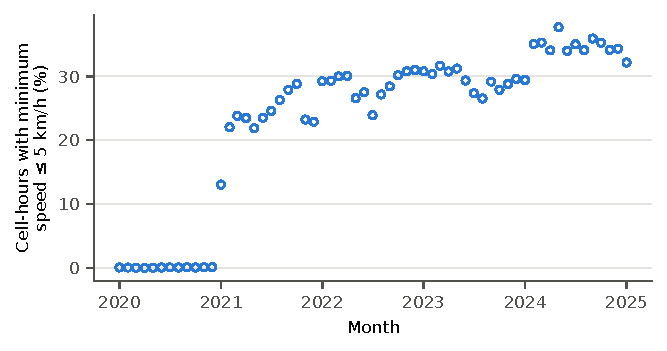
\includegraphics[width=.62\linewidth]{fig_speed_floor.pdf}
\caption{Share of cell-hours whose minimum recorded speed is 5~km/h or less, by month. The threshold
below which observations are discarded fell from about 6~km/h to 1~km/h in January 2021.}
\label{fig:floor}
\end{figure}

\subsection{Event dates and placebo dates}

The five commemorations fell on a Tuesday (2020), Wednesday (2021), Thursday (2022), Friday (2023)
and Sunday (2024). For each year the \emph{pool} contains 10 November and every other date of the same
weekday within eight weeks before and after. We remove public holidays, including the half day on
28 October, and the week of the schools' autumn break, which in these years began on the Monday
after 10 November.\footnote{Ministry of National Education calendars: 16--20 November 2020, 15--19
November 2021, 14--18 November 2022, 13--17 November 2023 and 11--15 November 2024. The data agree:
on the break-week date, speeds at 07:00--09:00 were \breakLo{}--\breakHi\% higher than on the
neighbouring same-weekday dates in 2021--2023.} The break matters because the date one week after the
event, the natural control in an adjacent-weeks design, falls inside it in four of the five years.
These rules were fixed before estimation. Table~\ref{tab:sample} gives the resulting sample:
\nDates{} dates, of which \nPlacebo{} are placebo dates.

\begin{table}[t]\centering
\caption{Sample by year. Cells are those observed on 10 November and on at least three quarters of
the pool dates. The lowest recorded speed is the first percentile of the minimum speed at 09:00.}
\label{tab:sample}
\Tab{sample}
\end{table}

\subsection{Other data}

Hourly precipitation and temperature for central Istanbul come from the Open-Meteo archive of
reanalysis weather. District boundaries come from OpenStreetMap, and district results of the 2024
metropolitan mayoral election from the tallies compiled in the Wikipedia article ``2024 Istanbul
mayoral election''. Neighbourhood (mahalle) results come from TÜİK's election statistics for two
elections: the 14 May 2023 parliamentary election, with party-list votes for 962 neighbourhoods, and
the 31 March 2024 metropolitan mayoral election, with votes for 960. We use the parliamentary vote
as the main measure, because it records party choice; the 2024 mayoral vote also reflects the
candidates and serves as a check. The CHP shares of the two elections correlate at 0.94 across
neighbourhoods. Neighbourhood
boundaries come from the land-registry (tapu kadastro) polygons; they follow the administrative
neighbourhoods closely but not exactly. Each cell receives the vote share of the neighbourhoods it
overlaps, weighted by area. We keep the \nCellsGeneral{} cells whose area is at least half covered by
neighbourhoods with a matched vote record (median coverage \medMatched\%); across these cells the
2023 CHP share has a standard deviation of \sdChpGeneral{} points. Finally, İBB's traffic index web
service returns a city-wide congestion index (1--99, higher is more congested) at five-minute
intervals for the latest 60 days. We saved the response on the evening of 10 November 2026; it
covers 11 September to 10 November 2026, and Section~\ref{sec:index} uses it to show what a
city-wide average hides and the cell-level design recovers. The hourly version of this index has
been used by \citet{alcan2022} and \citet{gulek2024}, who describes it as built from
camera-measured speeds on main roads.

\section{Method}

\subsection{Contrast, statistic and estimate}

Let $v_{gyd}(h)$ be the average speed in cell $g$ on date $d$ of year $y$ in the hour starting at
$h$. The within-day contrast is
\begin{equation}
c_{gyd} = \ln v_{gyd}(9) - \tfrac12\left[\ln v_{gyd}(8) + \ln v_{gyd}(10)\right].
\end{equation}
It is zero when the 09:00 hour lies on the line between its neighbours and negative when it dips
below. Anything that scales all three hours alike, such as rain all morning or a quiet day, cancels.
For each year we keep the cells $G_y$ observed on 10 November and on at least three quarters of the
pool dates, subtract each cell's mean contrast over the pool, and average over cells:
\begin{equation}
M_{yd} = \frac{1}{|G_y|}\sum_{g \in G_y} \left(c_{gyd} - \bar c_{gy}\right).
\end{equation}
All further steps use only these date-level numbers. The statistic for date $d$ is its difference
from the other $K_y - 1$ dates of its year, and the estimate is the mean over years of the statistic
on the event date $e_y$:
\begin{equation}
T_y(d) = M_{yd} - \frac{1}{K_y-1}\sum_{d' \neq d} M_{yd'}, \qquad
D = \frac{1}{5}\sum_{y} T_y(e_y).
\end{equation}
Years are weighted equally because each contributes one event.

Cells are grouped by their usual speed at 09:00, the mean over all pool dates of the year, into four
classes: below 30, 30--50, 50--70 and 70~km/h or more. The classes were set in a pilot analysis that
used three control dates per year. The grouping uses every pool date, the event date included, so
that it does not depend on which date is called the event. Section~\ref{sec:robust} reports a version
that classifies cells from other days altogether.

\subsection{Full-stop-equivalent minutes}\label{sec:minutes}

We report $m = 60\,(1 - e^{D})$. If each vehicle's speed is sampled at regular intervals and all
samples are averaged, the hourly mean is distance travelled divided by time, and a stop of $k$
minutes by a share $\pi$ of vehicles lowers it by the factor $1 - \pi k/60$. Then $m = \pi k$: the
minutes of standstill per vehicle. The assumption fails here, because samples below the threshold are
discarded. Suppose a vehicle brakes for $t_d$ minutes, stands for $s$ and accelerates for $t_a$.
With stationary samples removed, the average becomes distance over \emph{moving} time, which is
Wardrop's running speed, and
\begin{equation}
m \approx \pi\,\frac{t_d + t_a}{2}:
\end{equation}
the standing time $s$ disappears, and only the braking and restarting register. If speeds are
recorded when vehicles cross a point instead of at fixed intervals, the loss is smaller still, about
$\pi (t_d + t_a)/6$, because by Wardrop's identity a flow-weighted mean is blind to a full stop.
With ordinary braking and acceleration from 60~km/h, $t_d + t_a$ is about half a minute. These cases
are our own derivation from the definitions in \citet{wardrop1952} and \citet{herrera2010}; the
appendix gives the steps. Vehicles that slow to a crawl without stopping stay in the average under
every scheme.

We therefore read $m$ as a lower bound on the minutes of delay per vehicle, and we use three
features of the data to check the reading: the minimum speed in the hour should fall; the maximum
speed should not; and the number of distinct vehicles should not change.

\subsection{Inference}

The estimate rests on five event dates. However many cells are observed, the uncertainty in such a
design comes from shocks at the level of the date and does not shrink as cells are added
\citep{conley2011,ferman2019}. Standard errors computed from the cells, or clustered on the date
when only a handful of dates are treated, reject far too often, and bootstrap corrections fail when
a single cluster is treated \citep{mackinnon2017,mackinnon2018,bertrand2004}. That all cells of the
city are observed does not remove the uncertainty, which comes from which dates carry the event
\citep{abadie2020}. Reanalyses of published experiments show how much conventional inference can
overstate significance in designs with few effective observations \citep{young2019}. In our data the variance of a date's mean contrast is
\designEffect{} times what independent cells would give.

We therefore compare the event dates with placebo dates. Consider every assignment that picks one
date from each year's pool. For each we compute the mean over years of $T_y$, and the $p$-value is
the share of assignments whose value is as low as $D$ or lower, the observed one included. There are
\nAssign{} assignments and we enumerate them all. This is the logic of a randomization test with
years as blocks \citep{rosenbaum2002book,ernst2004,hess2017,athey2017}, of placebo tests in
comparative case studies \citep{abadie2010,abadie2015,firpo2018}, and of placebo tests over clusters,
which may be stretches of time \citep{hagemann2019}. The quantity estimated is the average effect
realized on the five event dates \citep{alvarez2023}. It is exact if, absent the siren, each date
of a pool were equally likely to produce any of the observed values. The date of the commemoration
is fixed by the calendar, not drawn at random, so this is an assumption, and the $p$-value is best
read as the significance of 10 November against a uniform benchmark over comparable dates
\citep{abadie2021,mackinnon2020}. It allows any dependence between cells within a date. It rules out
a trend across the weeks of the pool and dependence between neighbouring weeks. Permutation over
time is exact when the data are exchangeable under the null, and it over-rejects when a trend is left
in the comparison \citep{chernozhukov2021,roth2023}; we therefore check trend-adjusted versions.
Because the test is one-sided and uses a difference in means, it remains valid for the wider null
hypothesis that the siren raised speed on no date \citep{caughey2023}.

For intervals we invert the test: we subtract a hypothesized constant effect from the event dates
and keep the values that are not rejected at the 5\% level in either direction, which gives a 90\%
interval \citep{rosenbaum2002book,rosenbaum2002}. Without a constant effect the interval's lower end
bounds the largest yearly effect \citep{caughey2023}.

\paragraph{Regression version.} The comparison above uses only same-weekday dates. A fixed-effects
regression uses every day within eight weeks of the event and adds controls. For each year we
regress $\ln v_{gdh}$, hours 06 to 12, on cell-by-date effects, which absorb anything that moves a
cell's whole morning; cell-by-hour effects for each day type (Monday to Thursday, Friday, Saturday,
Sunday), which give each cell its usual hourly profile; hour effects for school-break days; and
hourly rainfall, a wet-hour indicator and temperature. The fixed effects and controls are partialled
out without the event, and the event statistic is formed from the residuals of the same-weekday pool
dates exactly as above. Under the null of no effect this is the covariance-adjusted randomization
test of \citet{rosenbaum2002}, so the placebo-date inference carries over unchanged. The regression
also gives each cell's response, which we regress on the district's vote share for each date to test
for a political gradient over the same assignments.

Four speed classes are tested, so we report $p$-values adjusted by the stepdown procedure of
\citet{romano2005b}, computed from the joint distribution of the four class statistics over the same
assignments. It controls the probability of any false rejection under the same assumption as the
single tests, and is less conservative than the Bonferroni and Holm corrections when the statistics
are positively dependent \citep{romano2005a}. A test of ``no effect in a class'' does not test
whether classes differ \citep{list2019,ding2016}, so we also test differences between classes
directly, over the same assignments. As a check that does not rely on comparing dates, we apply the sign-change test of
\citet{canay2017} to the five yearly estimates; with five years its smallest attainable one-sided
$p$-value is $1/32 = 0.031$. All computations use Python 3.12 with NumPy 2.3 and pandas 2.3.
Assignments are enumerated exactly when there are fewer than six million of them; for the largest
pool, two million are drawn at random.

\section{Results}

\subsection{Main estimates}

Table~\ref{tab:main} gives the estimates. Over all cells the effect on speed in the 09:00 hour is
$\estAll$ log points ($\times 100$), or \minAll{} full-stop-equivalent minutes, with a 90\% interval
from \ciAllLo{} to \ciAllHi{} minutes. The estimate is negative in \negAll{} of 5 years and its
$p$-value is \pAll. A slowdown of this size is what ordinary dates produce.

\begin{table}[t]\centering
\caption{Effect of the 10 November siren on speed in the 09:00 hour, 2020--2024. ``Effect'' is $D$,
the mean over years of the event date's contrast minus that of the placebo dates, in log points
$\times 100$. Full-stop minutes are $60(1 - e^{D})$. The interval inverts the two-sided placebo test.
$p$-values are one-sided shares of \nAssign{} assignments of one date per year; the stepdown
adjustment covers the four speed classes.}
\label{tab:main}
\Tab{main}
\end{table}

\begin{figure}[t]\centering
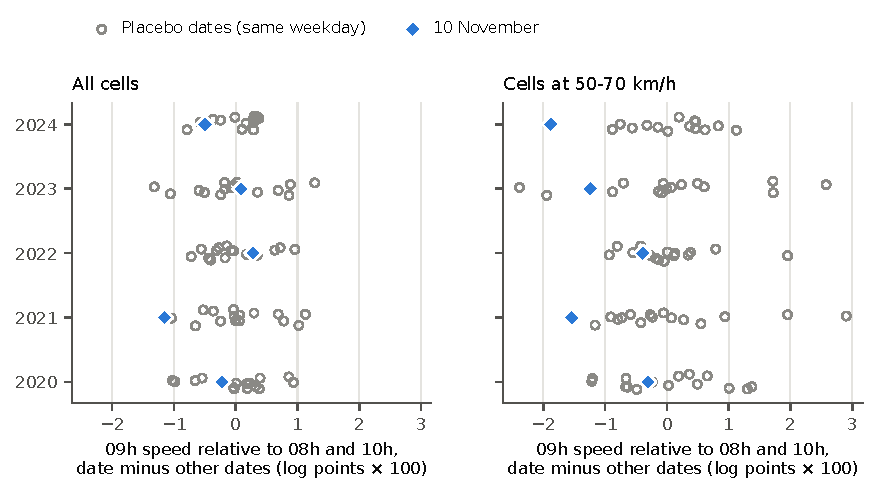
\includegraphics[width=.95\linewidth]{fig_placebo_dates.pdf}
\caption{The statistic $T_y(d)$ for each date of each year's pool: speed in the 09:00 hour relative to
the 08:00 and 10:00 hours, date minus the other dates of the year. Open circles are placebo dates of
the same weekday (vertical position jittered); diamonds are 10 November.}
\label{fig:placebo}
\end{figure}

The picture differs by class. In cells that usually flow at 50--70~km/h the effect is
$\estFast$, or \minFast{} minutes (90\% interval \ciFastLo{} to \ciFastHi), and it is negative in all
five years (Figure~\ref{fig:placebo}). Only a fraction \pFast{} of assignments give a value this
low; the stepdown-adjusted $p$-value is \pFastStep, and a joint test of the four classes gives
\pOmnibus. The sign-change test on the five yearly estimates gives \pFastSign, its minimum. The
other three classes are indistinguishable from ordinary dates: \minSlow{} minutes below 30~km/h,
\minMid{} at 30--50~km/h and \minMotor{} at 70~km/h or more. The differences between
the 50--70 class and these three have one-sided $p$-values of \pDiffSlow, \pDiffMid{} and
\pDiffMotor. The yearly estimates for this class
range from \minFastYearLo{} minutes in \yearFastLo{} to \minFastYearHi{} in \yearFastHi{} (Appendix
Table~\ref{tab:years}).

Figure~\ref{fig:profile} shows the estimate in ten-km/h bands. It is largest in the 50--60 band
(\minBinFifty{} minutes, $p = \pBinFifty$), smaller and not significant by itself in the 60--70 band (\minBinSixty{} minutes,
$p = \pBinSixty$), and within the range of placebo dates everywhere else.

\begin{figure}[t]\centering
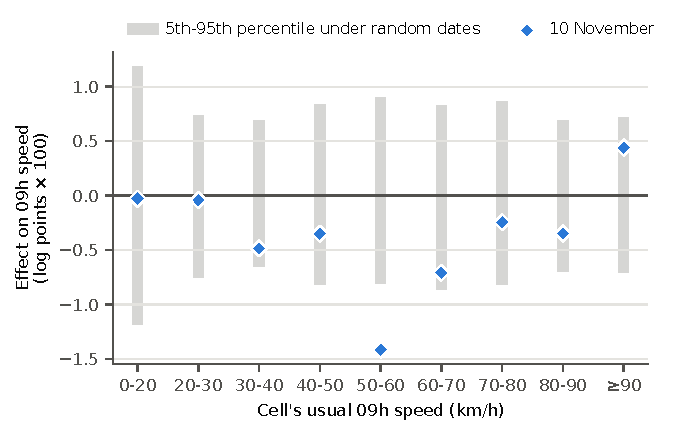
\includegraphics[width=.66\linewidth]{fig_speed_profile.pdf}
\caption{Effect on speed in the 09:00 hour by the cell's usual speed at 09:00. Diamonds are the
estimates for 10 November; grey bars span the 5th to 95th percentile of the same statistic over
assignments of one date per year. One log point $\times 100$ is about 0.6 full-stop-equivalent
minutes.}
\label{fig:profile}
\end{figure}

\subsection{Minimum speed, maximum speed and vehicles}

If vehicles brake to a halt and restart, the slowest observation in the hour should be slower, the
fastest should not change, and the number of distinct vehicles should not change. Table~\ref{tab:out}
shows this pattern. The minimum speed in the 09:00 hour fell by \minspFastPct\% in the 50--70 class
($p = \pMinspFast$) and by \minspAllPct\% over all cells ($p = \pMinspAll$, negative in \negMinspAll{}
of 5 years). The maximum speed and the number of vehicles did not move in either group. In
2021--2024, when the threshold was 1~km/h, the share of 50--70 cells whose minimum speed was
2~km/h or less rose by \floorShareFast{} percentage points in the 09:00 hour ($p = \pFloorShareFast$).

\begin{table}[t]\centering
\caption{Other outcomes and placebo tests. Each row applies the main design to another outcome, hour
or date. Effects are in log points $\times 100$, except the share of cells (percentage points). ``Years''
counts years with a negative estimate (positive for the share). $p$-values are one-sided in the
direction of a slowdown.}
\label{tab:out}
\Tab{outcomes}
\end{table}

\subsection{Other hours and other days}

The same contrast can be formed for any hour: speed in hour $h$ relative to hours $h-1$ and $h+1$.
Figure~\ref{fig:hours} shows it for the 50--70 class. The 09:00 hour gives
$\curNine$ ($p = \pCurNine$). The 08:00 and
10:00 values are raised mechanically, since each uses the 09:00 hour as a reference. The 10:00 value
($\curTen$) is higher than this mechanical share alone would give, which indicates that the 10:00
hour was itself fast on 10 November. The 09:00 hour is not alone: of the \nHours{} hours,
\nHoursLow{} (\hoursLowList) fall below the 5th percentile of their placebo distribution, against
one expected by chance. Contrasts centred on 07:00
and 11:00, which do not involve the 09:00 hour, are not significant in the 50--70 class
($p = \pPlacSevenFast$ and \pPlacElevenFast); over all cells the 11:00 contrast is negative
($p = \pPlacElevenAll$). Moving the ``event'' to 9 or 11 November gives nothing (Table~\ref{tab:out}).

\begin{figure}[t]\centering
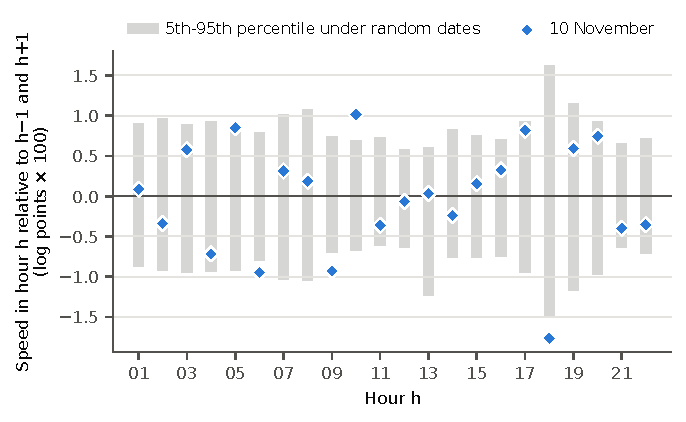
\includegraphics[width=.68\linewidth]{fig_hour_curvature.pdf}
\caption{Speed in each hour relative to the hours before and after it, 10 November minus placebo
dates, cells at 50--70~km/h. Diamonds are the estimates; grey bars span the 5th to 95th percentile
over assignments of one date per year. Hours 08 and 10 are raised mechanically by the dip at 09.}
\label{fig:hours}
\end{figure}

\subsection{Which hour moves}

The contrast compares the 09:00 hour with its two neighbours, so a fast neighbour and a slow 09:00
hour look alike. To separate them we measure each of the three hours against the mean of the hours
06, 07, 11 and 12, none of which adjoins the siren. In the 50--70 class the 08:00 hour is ordinary
on 10 November ($\estEightFast$, $p = \pEightFast$). The 10:00 hour is fast: $+\estTenFast$ log
points ($\times 100$), positive in \posTenFast{} of 5 years, with a one-sided $p$-value of
\pTenFast{} in that direction. The 09:00 hour is slow by $\estNineFar$, or \minRobFar{} minutes,
negative in \negRobFar{} of 5 years ($p = \pRobFar$). So the main estimate has two parts: a 09:00
hour that is slower than distant hours by about \minRobFar{} minutes, and a 10:00 hour that is
faster than usual. The minimum speed shows the
same split. Against the 08:00 hour alone it is lower at 09:00 by \minspPreFast\%
($p = \pMinspPreFast$); against the 10:00 hour alone, by \minspPostFast\% ($p = \pMinspPostFast$;
Table~\ref{tab:out}). The fast 10:00 hour has two candidate explanations: it belongs to the
event, as a release after the stop or as lighter traffic after the ceremonies, or it is a feature of
the day unrelated to the siren.

\subsection{Regression with fixed effects and weather}

Table~\ref{tab:reg} gives the regression version. In the 50--70 class the 09:00 hour is slower
than its neighbours by \regMainFast{} minutes, negative in \negRegMainFast{} of 5 years
($p = \pRegMainFast$). Without the weather controls the figure is \regNoCtlFast{}
($p = \pRegNoCtlFast$), so rain and temperature account for a small part of the main estimate.
Against hours that do not adjoin the siren the regression gives \regFarFast{} minutes
($p = \pRegFarFast$), and against the 08:00 hour \regPreFast{} ($p = \pRegPreFast$). The
regression thus confirms both the slowdown relative to the neighbouring hours and its dependence on
the fast 10:00 hour. Over all cells the estimates stay small (\regMainAll{} minutes,
$p = \pRegMainAll$).

\begin{table}[t]\centering
\caption{Fixed-effects regression version. Cell-by-date and cell-by-day-type-by-hour fixed effects,
school-break hour effects, and hourly rain and temperature are partialled out over all days within
eight weeks of 10 November; the event statistic is formed from the residuals of same-weekday pool
dates. Minutes are full-stop-equivalent minutes; $p$-values are one-sided placebo-date $p$-values.}
\label{tab:reg}
\Tab{regression}
\end{table}

\subsection{Where}\label{sec:het}

Within the 50--70 class the estimate is \minEurope{} minutes on the European side and \minAsia{} on
the Asian side, and the difference is far from significant ($p = \pSideDiff$;
Table~\ref{tab:het}). Splitting the cells by the district's vote for the Republican People's Party
(CHP) candidate in the 2024 mayoral election gives \minChpLow, \minChpMid{} and \minChpHigh{}
minutes from the lowest to the highest band of vote share, with no significant difference between groups (smallest
$p = \pChpDiffMin$). Across the \nDistricts{} districts with enough cells, the estimate is
negative in \nDistNeg{} and its correlation with the CHP share is \corrChp{}
(Appendix Figure~\ref{fig:districts}). Cells with few and
many probe vehicles give similar estimates.

On slower roads the vehicles in a cell are more likely to belong to the surrounding area, so the
local vote is a closer proxy for the drivers there than on arterials and motorways that pass
through. Table~\ref{tab:pol} reports, for each speed class, the slope of the cell-level response on
the CHP share (standardized over cells), from the regression residuals, with placebo-date
$p$-values, once with the district share and once with the neighbourhood share.

District shares show no consistent gradient: \nSigDistrict{} of the ten slopes has a two-sided
$p$-value below 0.05. Neighbourhood shares, which match the size of a cell, show one. With the 2023
parliamentary vote, cells below 30~km/h in neighbourhoods with a higher CHP share slow more in all
five years: by $\slopeGeneralMainSlow$ log points ($\times 100$) per standard deviation against the
neighbouring hours ($p = \pSlopeGeneralMainSlow$) and by $\slopeGeneralFarSlow$ against hours that do
not adjoin the siren ($p = \pSlopeGeneralFarSlow$). Adjusted for the ten slopes tested these become
\pSlopeGeneralMainSlowHolm{} and \pSlopeGeneralFarSlowHolm. The 2024 mayoral vote gives the same
pattern, slightly stronger ($p = \pSlopeNeighbourhoodMainSlow$ and \pSlopeNeighbourhoodFarSlow). In
the 50--70 class the slope is negative in all five years against the neighbouring hours
($\slopeGeneralMainFast$, $p = \pSlopeGeneralMainFast$), and over all cells it is negative against
the distant hours in all five years ($p = \pSlopeGeneralFarAll$). Motorway cells show no gradient.
The European and Asian sides do not differ in any class (smallest $p = \pSideRegMin$).

A standard deviation of the neighbourhood CHP share is \sdChpGeneral{} percentage points in 2023. In slow
cells the average response is close to zero, so the gradient implies a slowdown at 09:00 in
neighbourhoods with a high CHP share and a small speed-up, or none, in neighbourhoods with a low one.

\begin{table}[t]\centering
\caption{Political gradient. Slope of the cell-level event response on the CHP vote share (standardized over
cells): district share in the 2024 mayoral election, and neighbourhood shares in the 2023
parliamentary and 2024 mayoral elections, by usual 09:00 speed, in log points
$\times 100$ per standard deviation. A negative slope means a larger slowdown where the CHP
share is higher. Superscripts count the years (of five) with a negative slope. $p$-values are
two-sided placebo-date $p$-values. The neighbourhood share of a cell is area-weighted over the
neighbourhoods it overlaps.}
\label{tab:pol}
\Tab{politics}
\end{table}

\begin{table}[t]\centering
\caption{Estimates for groups of cells within the 50--70~km/h class.}
\label{tab:het}
\Tab{heterogeneity}
\end{table}

\subsection{Comparison with a city-wide index}\label{sec:index}

A single city-wide series hides the disturbance that the cell-level design finds.
Figure~\ref{fig:index} shows İBB's traffic index at five-minute intervals on the morning of
10 November 2026, a Tuesday, against the other \idxN{} working days of the preceding two months. The
index averages over the whole network, in which the cells that flow at 50--70~km/h are
\shareFast\% of all cells, and it shows no rise at 09:05. The statistic analogous to the hourly
contrast, the index in the two five-minute readings after 09:00 minus the mean of the readings
twenty minutes earlier and later, is \idxStat{} index points on 10 November, against a mean of
\idxCtrlMean{} and a standard deviation of \idxCtrlSd{} on the other days; it ranks \idxRank{} of
\the\numexpr\idxN+1\relax{} ($p = \idxP$). We chose this window after seeing the series; windows of
fifteen and thirty minutes give ranks of \idxRankShort{} and \idxRankLong. Grouping cells by their
usual speed is what isolates the arterial roads on which the 09:00 hour is slow, and a finer time
step applied to an average over all roads does not replace it.

\begin{figure}[t]\centering
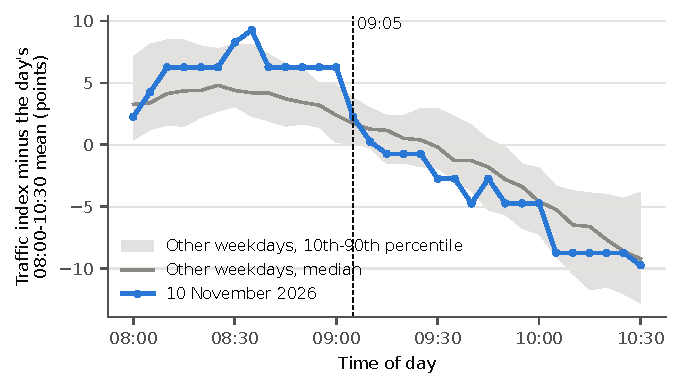
\includegraphics[width=.68\linewidth]{fig_index_2026.pdf}
\caption{İBB city-wide traffic index (higher is more congested) at five-minute intervals on
10 November 2026 and on the other working days from 14 September to 9 November 2026, each day
measured from its own mean between 08:00 and 10:30.}
\label{fig:index}
\end{figure}

\section{Robustness}\label{sec:robust}

Table~\ref{tab:rob} repeats the analysis under other choices, for all cells and for the 50--70 class.
Of the \nRobSpecs{} specifications for the 50--70 class, \nRobSig{} give a $p$-value below 0.05. The
three that do not are the three that avoid the 10:00 hour as a reference.

\begin{table}[p]\centering
\caption{Robustness. Each row changes one feature of the main specification. Minutes are
full-stop-equivalent minutes; $p$-values are one-sided placebo-date $p$-values; ``Years $<0$'' counts
years with a negative estimate.}
\label{tab:rob}
\Tab{robustness}
\end{table}

\paragraph{Placebo-date pool.} With the three control dates of the pilot (3, 17 and 24 November)
the 50--70 estimate is \minRobPilot{} minutes ($p = \pRobPilot$), and with the two adjacent weeks
alone \minRobAdjacent{} ($p = \pRobAdjacent$). Pools of four, eight and twelve weeks on each side
give \minRobFour, \minFast{} and \minRobTwelve{} minutes, every same-weekday date of the calendar
year gives \minRobYear{} ($p = \pRobYear$), and keeping the school-break dates gives
\minRobBreak. Across these pools the estimate lies between \minPoolLo{} and \minPoolHi{} minutes
and the $p$-value never exceeds \pPoolMax. In contrast with the election-day and 20 April studies
\citep{zhang2016,harper2019}, widening the pool leaves the result for this class in place. It
removes the result for the 30--50 class, whose pilot $p$-value of 0.034 becomes \pMid{}
(\pMidStep{} after adjustment).

\paragraph{Trend and scale.} Removing a linear or quadratic trend in $M_{yd}$ across the weeks of
each year, fitted without the date under test, gives \minRobTrend{} and \minRobQuad{} minutes. A
raw difference in means can mislead when the event dates are more variable than the others
\citep{chung2013,wu2021}. Dividing each year's statistics by the standard deviation of its placebo
dates gives $p = \pRobZ$, and replacing them by ranks gives $p = \pRobRank$. Removing the part of
$M_{yd}$ explained by rain and temperature, in the manner of \citet{rosenbaum2002}, gives
\minRobRain{} minutes.

\paragraph{Reference hours.} This is where the estimate is fragile. Against the 08:00 hour alone
it is \minRobPre{} minutes ($p = \pRobPre$); against the 10:00 hour alone, \minRobPost{}
($p = \pRobPost$). Against the four hours 07, 08, 10 and 11 it is \minRobWide{} ($p = \pRobWide$),
and against the hours 06, 07, 11 and 12, none of which adjoins the event, \minRobFar{}
($p = \pRobFar$). Subtracting the mean contrast at the placebo hours 07 and 11 gives
\minRobNet{} ($p = \pRobNet$). The contrast against the earlier hour is the cleanest in principle,
because the later hour comes after the event \citep{rosenbaum2002book}; it is also the weakest.
A fast hour after a synchronized pause has been seen elsewhere \citep{meier2014,ngeni2022}, but
here it comes a full hour later, and we do not attribute it to the stop.

\paragraph{Cells and classification.} Restricting to cells observed on every pool date, or to cells
with at least ten probe vehicles, gives \minRobBalanced{} and \minRobTen{} minutes. Weighting cells by their number of probe
vehicles gives \minRobWeighted{} minutes ($p = \pRobWeighted$). An earlier version of the analysis classified cells by their speed on the placebo dates only;
it gave a somewhat larger estimate and was replaced, because it treats the event date differently
from the others. Classifying cells by their speed on
days outside the pool, so that classification and estimation share no data, gives a smaller estimate
of \minRobOther{} minutes ($p = \pRobOther$), negative in all five years. Some of the difference is
the dilution that comes with a noisier classification; some may be selection on the same noisy speeds
that enter the contrast, and we regard this estimate as the more cautious one.

\paragraph{Years.} Leaving out one year at a time gives between \minLooLo{} and \minLooHi{} minutes,
with $p$-values of at most \pLooMax. Without 2024, when the event fell on a Sunday, the estimate is
\minRobWeekday{} minutes. Without 2020, the year of the higher speed threshold and of pandemic
restrictions, it rises to \minLooHi.

\paragraph{Sensitivity and power.} Following \citet{rosenbaum2002book}, we ask how far the uniform
benchmark must fail before the conclusion changes. If within each year the odds of being the event
date could differ between dates by a factor $\Gamma$, the worst-case $p$-value for the 50--70 class
stays below 0.05 up to $\Gamma = \gammaMax$. To gauge what the design can detect, we lowered the
statistic of one randomly chosen placebo date per year by the effect of a full stop of given length
and reran the test. A stop equivalent to half a minute is detected at the 5\% level in \powerAllHalf\%
of simulations over all cells and \powerFastHalf\% in the 50--70 class; one of a quarter of a minute in
\powerAllQuarter\% and \powerFastQuarter\%. The small estimate over all cells is therefore informative:
a measured slowdown of half a minute across all cells would very probably have been found.

\section{Discussion}

\paragraph{What the data show.} On roads that normally flow at 50--70~km/h, the hourly profile of
10 November is unusual around the siren in every one of five years: the 09:00 hour lies below the
line between its neighbours by an amount that few random choices of dates would produce. The 09:00
hour is slower than more distant hours by about \minRobFar{} minutes, the minimum speed falls and
the maximum does not, as braking and restarting would imply. The rest of the gap comes from a fast
10:00 hour. We read this as evidence of a disturbance at the siren on these roads, with a size
between \minRobFar{} and \minFast{} full-stop-equivalent minutes.
The pattern does not depend on the side of the city. At the level of districts it does not depend
on politics either, which fits \citeauthor{goldman2018}'s (\citeyear{goldman2018}) account of a
commemoration shared across camps. At the level of neighbourhoods it does: on slow, local streets,
the slowdown rises with the CHP vote, the secular profile that \citet{ozyurek2004} associates with
voluntary Atatürk commemoration. Districts mix neighbourhoods of different leanings, and arterial
traffic mixes drivers from across the city; the neighbourhood gradient on local streets is the
comparison in which drivers and voters coincide most closely.

\paragraph{Why only there.} The estimate is absent below 50~km/h and above 70~km/h. Studies of
demand shocks find larger effects on more congested roads \citep{adler2021,hanna2017}; we find the
opposite at the slow end. The measurement explains part of this. Where traffic already stops and
starts, standing is routine, the average is already a running speed, and a further stop adds little
that the data retain. At the fast end, cells with a usual speed above 70~km/h are motorways, where
stopping in a live lane is dangerous and may be rarer. Lower participation and weaker measurement
both predict this pattern.

\paragraph{What the minutes mean.} If the published average were distance over time for all
vehicles, half a minute would be the standstill per vehicle: half of the vehicles stopping for one
minute, or fewer for longer. The threshold in the data rules this reading out. If instead only
moving vehicles are averaged, full compliance with ordinary braking would produce between about 0.15
and 0.35 minutes. Our estimates, from \minRobPre{} to \minRobPost{} minutes depending on the reference hour, lie at
the top of that range or above it, so they contain more than clean stops:
crawling vehicles and slow restarts of platoons enter, and so, in the main contrast, does the fast
10:00 hour. The smaller estimate for 2020 (\minFastTwenty{} minutes), when observations below
6~km/h were discarded, is in line with this; 2020 was also a year of pandemic restrictions. In comparable units the effect is small: about 1\% of travel time in the hour, a tenth or
less of what a one-day transit strike adds in the morning peak
\citep{bauernschuster2017,anderson2014}.

\paragraph{Scope.} The estimate rests on five events and on one of four speed classes, chosen in
a pilot on the same five event dates; the wider pool of placebo dates is the new evidence. It varies
with the reference hour between \minRobPre{} and \minRobPost{} minutes, and the versions that avoid
the 10:00 hour have $p$-values between \pRobFar{} and \pRobPre. Ceremonies at 09:05 in schools and
offices shift trips on the day. The estimates are full-stop-equivalent minutes of measured speed,
a lower bound on the delay per vehicle.

\paragraph{Extension.} The same placebo-date design applies directly to speeds recorded every
minute on arterial segments from 08:45 to 09:30 on 10 November and on comparison days. İBB's own
sensors record at this resolution \citep{takak2021}. At that resolution the stop appears as a dip
of measured depth and length, and the release after it is observed directly.

\section{Conclusion}

In hourly open data, Istanbul's remembrance stop leaves a trace only where traffic normally flows
freely on arterial roads. There the 09:00 hour of 10 November lies below its neighbours in every
year, by the equivalent of \minFast{} minutes of full stop per vehicle; measured against more
distant hours the figure is \minRobFar{} minutes and is no longer statistically distinguishable from
an ordinary date. Both are lower bounds, because standing vehicles are missing from the data.
Averaged over the whole city the hour is not measurably slower than on any other day, and the design
would probably have detected half a minute. The design that finds this, a within-day contrast judged
against a wide pool of placebo dates, guards against the failures documented for adjacent-week
comparisons, and it locates the disturbance on the roads where it occurs, which an average over the
whole city hides. Minute-level speeds on the same roads on the next 10 November extend the design to
the depth and length of the stop.

\section*{Data and code}
All data are public. Code to download the data and reproduce every number, table and figure is at
\url{https://github.com/msamiboz/saygi-durusu-traffic}. Numbers in the text are generated by the code.

\bibliographystyle{plainnat}
\bibliography{references}

\appendix
\section{Yearly estimates}

\begin{table}[h]\centering
\caption{Yearly estimates $T_y(e_y)$ by speed class, log points $\times 100$.}
\label{tab:years}
\Tab{years}
\end{table}

\begin{figure}[h]\centering
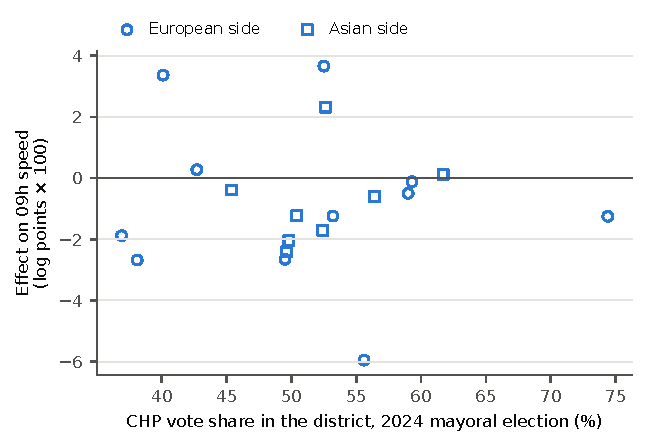
\includegraphics[width=.62\linewidth]{fig_districts.pdf}
\caption{District estimates for cells at 50--70~km/h against the district's vote share for the CHP
candidate in the 2024 metropolitan mayoral election. Circles are districts on the European side,
squares on the Asian side. Districts with fewer than five such cells in any year are omitted.}
\label{fig:districts}
\end{figure}

\section{What an hourly mean retains of a brief stop}\label{app:schemes}

Consider one cell and one hour with baseline speed $v_0$. A share $\pi$ of vehicles brakes linearly
for $t_d$ minutes, stands for $s$ minutes and accelerates linearly for $t_a$ minutes. Each loses the
distance $v_0 k^*$, where $k^* = s + (t_d + t_a)/2$ is the full-stop-equivalent duration.

\emph{(A) Speeds sampled at fixed time intervals, all samples kept.} Samples are proportional to
vehicle-time, so the mean is total distance over total time, $v_0(1 - \pi k^*/60)$, and
$60(1 - e^{D}) = \pi k^*$.

\emph{(B) Fixed intervals, stationary samples discarded.} The same distance is divided by moving time,
$60 - \pi s$. The mean is $v_0 (60 - \pi k^*)/(60 - \pi s)$ and
$60(1 - e^{D}) \approx \pi (t_d + t_a)/2$.

\emph{(C) Speeds recorded on crossing a point.} The mean is flow-weighted. By the identity
$v_t = v_s + \sigma_s^2/v_s$ of \citet{wardrop1952}, a population that spends a fraction $s/60$ of the
hour at zero speed and the rest at $v_0$ has space-mean speed $v_0(1 - s/60)$ and time-mean speed
exactly $v_0$. Only the ramps register, with a loss of about $\pi(t_d + t_a)/6$.

\emph{(D) One speed per traversal of the cell, averaged over vehicles.} If a free traversal takes
$\tau$ minutes, a share $\tau/60$ of the hour's traversals meets the stop, each at speed
$v_0\tau/(\tau + k^*)$, so $60(1 - e^{D}) \approx \pi \tau k^*/(\tau + k^*)$, which is below both
$\tau$ and $k^*$.

Scheme A predicts the same minutes in every speed class; B predicts minutes proportional to speed,
since $t_d + t_a$ is; D predicts more minutes in slower cells. The data show none of these
gradients (Figure~\ref{fig:profile}), a minimum speed that is never zero, an unchanged number of
vehicles, and a lower minimum speed in the event hour. Schemes B and C, with some crawling vehicles,
are the readings most in line with these facts.

\end{document}
